\paragraph{\trHochschildCohomology{}计算。}\label{sub:hochschild-computation}
我们不去直接对 $A$ 上的\trAinfty{}结构进行分类，而是宁愿暂时转到一个略大一些的代数 $\bar{A}$ 上去。它是扩充后的（比原来多一个\trVertex{}的）\trQuiver
\begin{equation}\label{eq:extended-quiver}
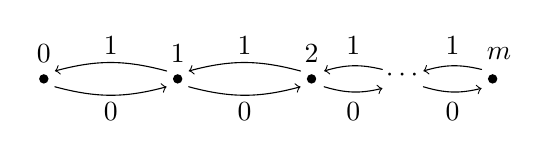
\begin{tikzpicture}[line cap=round,line join=round]
\fill (0,0) circle (1.7pt);
\node at (0,0.32) {$0$};
\fill (1.7,0) circle (1.7pt);
\node at (1.7,0.32) {$1$};
\fill (3.4,0) circle (1.7pt);
\node at (3.4,0.32) {$2$};
\node at (4.55,0.05) {$\cdots$};
\fill (5.7,0) circle (1.7pt);
\node at (5.78,0.32) {$m$};
\draw[->] (1.56,0.1) to[bend right=15] (0.14,0.1);
\node at (0.85,0.42) {$1$};
\draw[->] (0.14,-0.1) to[bend right=15] (1.56,-0.1);
\node at (0.85,-0.42) {$0$};
\draw[->] (3.26,0.1) to[bend right=15] (1.84,0.1);
\node at (2.55,0.42) {$1$};
\draw[->] (1.84,-0.1) to[bend right=15] (3.26,-0.1);
\node at (2.55,-0.42) {$0$};
\draw[->] (4.3,0.12) to[bend right=15] (3.56,0.1);
\node at (3.93,0.42) {$1$};
\draw[->] (3.56,-0.1) to[bend right=15] (4.3,-0.12);
\node at (3.93,-0.42) {$0$};
\draw[->] (5.56,0.12) to[bend right=15] (4.82,0.1);
\node at (5.19,0.42) {$1$};
\draw[->] (4.82,-0.1) to[bend right=15] (5.56,-0.12);
\node at (5.19,-0.42) {$0$};
\end{tikzpicture}
\end{equation}
对关系
\begin{equation*}
\begin{gathered}
(i+2,i+1,i)=0,\qquad (i-2,i-1,i)=0,\\
(i,i+1,i)+(i,i-1,i)=0,\qquad (0,1,0)=0
\end{gathered}
\end{equation*}
所取的商。由构造，$\bar{A}$ 在 $\bar{R}=\KK^{m+1}$ 上是\trLinear{}的。也许令人意外的是，这个扩大后的代数比 $A$ 性状更好：它具有有限的\trCohomology{}维数，并且还是一个\trKoszul{}代数。我们现在就来解释后一性质的含义。
由于 $\bar{A}$ 是一个\trPathAlgebra{}对（按\trDegree{}与路径长度而言齐次的）理想所取的商，$\bar{A}$ 便又一次带有一个双\trGrading。于是，Ext 代数
\begin{equation}\label{eq:ext-algebra}
\operatorname{Ext}_{\bar{A}}(\bar{R},\bar{R})
\end{equation}
\trApriori{}地是三\trGraded{}的（按\trCohomology\trDegree；按由 $\bar{A}$ 中诸元素的\trDegree{}导出的内蕴\trGrading；最后按长度\trGrading——它同样是经由 $\bar{A}$ 中相应的\trGrading{}导出的）。如果取 \eqref{eq:ext-algebra} 底下的约化 bar 构造，那么显然上链的\trCohomology\trGrading{}总不超过其长度\trGrading。此外，\trCochainComplex{}中这两个\trGrading{}彼此相合的那一部分可以被显式地描述。这样得出的结果如下。设 $\bar{A}^*$ 是 $\bar{A}$ 的\textbf{\trQuadraticDual{}}（quadratic dual）。它具有\trGenerator{}$(i,1\pm 1)^*$，与 $(i\pm 1,i)$ 对偶，其\trDegree{}为 $|(i,i\pm 1)^*|=1-|(i\pm 1,i)|$，并且带有关系
\begin{equation*}
(i,i+1,i)^*+(i,i-1,i)^*=0,\qquad (m,m-1,m)^*=0.
\end{equation*}
然后，取 bar 上链并把它们限制到\trGenerator{}$(i\pm 1,i)$ 上，就定义了一个\trCanonical\trHomomorphism
\begin{equation}\label{eq:ext-to-quaddual}
\operatorname{Ext}_{\bar{A}}(\bar{R},\bar{R})\longrightarrow\bar{A}^*.
\end{equation}
在我们的情形，从 [85, Proposition 2.1] 所给出的单模的投射分解可知，Ext 代数的这个三\trGrading{}是部分对角的，也就是说，所有非零分片都具有其\trCohomology\trGrading{}与长度\trGrading{}相合的性质。这恰恰就是\trKoszul{}代数的性质——在 [110] 的意义下（略作推广，因为我们以\trSemisimple{}环 $\bar{R}$ 而不是一个域作为基）。它\trEquivalence{}于 \eqref{eq:ext-to-quaddual} 为\trIsomorphism。
接下来，我们考虑 $\bar{A}$ 的约化\trHochschild\trCochainComplex，它由从 $\bar{A}/\bar{R}$ 到 $\bar{A}$ 的\trMultilinear{}映射组成。可以按映射目标上的路径长度对这个\trComplex{}进行\trFiltration，所得的便是一个\trSpectralSequence，其 $E_1$ 页可以写成
\begin{equation}\label{eq:spectral-e1}
\operatorname{Ext}_{\bar{A}}(\bar{R},\bar{R})\otimes_{\bar{R}\otimes\bar{R}}\bar{A}\cong
\bar{A}\otimes_{\bar{R}\otimes\bar{R}}\bar{A}^*.
\end{equation}
由于 $\bar{A}$ 及其对偶都是有限维的，这个\trSpectralSequence{}显然\trConvergence{}于 $HH(\bar{A},\bar{A})$。形象地说，$E_1$ 页上的\trGenerator{}可以想成由两段构成的闭路径，这两段分别位于 \eqref{eq:extended-quiver} 的\trQuiver{}及其对偶之中。具体地，它们可以写成表达式
\begin{equation}\label{eq:e1-generators}
(i_l,\ldots,i_0)\otimes(j_0,\ldots,j_r)^*
\quad\text{其中 } j_r=i_l,\ j_0=i_0.
\end{equation}
\trGrading{}方面的问题可以按如下方式理清。假设我们感兴趣的是 $HH^{r+s}(\bar{A},\bar{A})^s$，它是由内蕴\trDegree{}为 $s$ 的 $r$-\trLinear\trHochschild\trCocycle{}所表示的群（这一记号与\cref{sub:length-filtration}中的相同）。于是，\eqref{eq:spectral-e1} 中起贡献的项由这样一些表达式 \eqref{eq:e1-generators} 组成：其 $r$ 已给定，并且满足 $|(j_0,\ldots,j_r)^*|+|(i_l,\ldots,i_0)|=r+s$。由于我们这些\trQuiver{}的\trGrading{}方式，此时便得到 $l=2s+r$。
\begin{lemma}\label{thm:extended-hh-pieces}
$HH^2(\bar{A},\bar{A})^{2-r}$ 当 $r\ge 5$ 时为零，当 $r=3$ 时也为零，而当 $r=4$ 时为 $\KK$。\footnote{译注：原书此处印作“is zero for $r\le 5$”；疑应为“$r\ge 5$”（同页证明梗概首句正以 $l=4-r<0$ 论证 $r\ge 5$ 时消没，且本条目自身又设 $r=4$ 处取 $\KK$，与“$r\le 5$ 时为零”内相矛盾）；此处径改。——译者注}
\end{lemma}
\begin{proof}[证明梗概]
这对 $r\ge 5$ 是直截了当的，因为起贡献的项 \eqref{eq:e1-generators} 将需要 $l=4-r<0$。$r=3,4$ 的情形要略微复杂一些：我们略去细节，但为以后使用记录一个推论。\eqref{eq:spectral-e1} 的边\trHomomorphism{}给出一个映射
\begin{equation}\label{eq:edge-homomorphism}
HH^2(\bar{A},\bar{A})^{-2}\longrightarrow
\bar{R}\otimes_{\bar{R}\otimes\bar{R}}(\bar{A}^*)^2.
\end{equation}
这里，目标空间由 $\bar{A}^*$ 中\trDegree{}为二的元素组成，$\bar{R}$ 的诸\trIdempotent{}（以从左从右相同的方式）对角地作用于其上。从这个计算可以看出，\eqref{eq:edge-homomorphism} 是\trInjective{}的，并且它的像由（$\bar{A}^*$ 的中心元）
\begin{equation}\label{eq:central-element}
(0,1,2,1,0)^*+(1,2,3,2,1)^*+\cdots+(m-2,m-1,m,m-1,m-2)^*
\end{equation}
的倍数组成。
\end{proof}
着眼于一般的分类理论，\cref{thm:extended-hh-pieces} 蕴含：在固定\trCohomology{}的\trQuasiisomorphism{}之下，使 $H(\bar{\scr{A}})\cong\bar{A}$ 的\trACategory{}$\bar{\scr{A}}$ 至多构成一个单参数族。把这个参数记作 $q\in\KK$（$q=0$ 对应于形式的\trAinfty{}结构）。\cref{thm:extended-hh-pieces} 本身并未给出非形式结构存在性的证明——那种结构将对应于 $q\ne 0$ 的值（实际上，不同的非零值可以通过对各个\trGraded{}分片的\trRescaling{}而相互关联，所以它们并没有实质性的差异）。不过，暂且假定这种结构确实存在，那么可以安排得使它们的首个非平凡高阶乘积是 $\mu^4$。此外，从 \eqref{eq:central-element} 可知，对 $m\ge 5$，这个乘积将满足 \eqref{eq:mu4-combination} 的一个取非零 $q$ 的类似式。特别地，如果此时把对应于那个额外\trVertex{}的\trObject{}丢弃，所得的\trFullSubcategory{}仍将借\cref{thm:surface-nonformality-lemma}而是非形式的。
